\chapter{The Design And Development Of CIPRNG}
\label{CI dev}
\minitoc

In this chapter, some studies for CIPRNG algorithm are given. 
First of all, some researches of Version 1 CI are deepen. Then
the designs of our three new versions of CI pseudo random number generators based 
on discrete chaotic iterations, satisfying Devaney's chaos, are proposed and discussed.
Detail operations of this approach are described in this chapter, 
while their performance and a comparative study will be presented latter.



\section{Development of Version 1 CI Algorithm}

\subsection{On the periodicity of chaotic orbit}
\label{Conclusions and Future Work}
\label{Experiments and statistical tests}

Since chaotic iterations are constrained in a discrete space with $2^{N}$ elements, it is obvious that every chaotic orbit will eventually be periodic, i.e., finally goes to a cycle with limited length not greater than $2^{N}$.

The schematic view of a typical orbit of a digital chaotic system is shown in Figure~\ref{A pseudo orbit of a digital chaotic system}. Generally speaking, each digital chaotic orbit includes two connected parts: $x^{0} , x^{1} , \dots, x^{l-1}$ and $ x^{l} , x^{l +1} , \dots , x^{l +n}$ , which are respectively called transient (branch) and cycle. Accordingly, $l$ and $n + 1$ are respectively called transient length and cycle period, and $l + n$ is called orbit length. Thus,

\begin{figure}
\centering
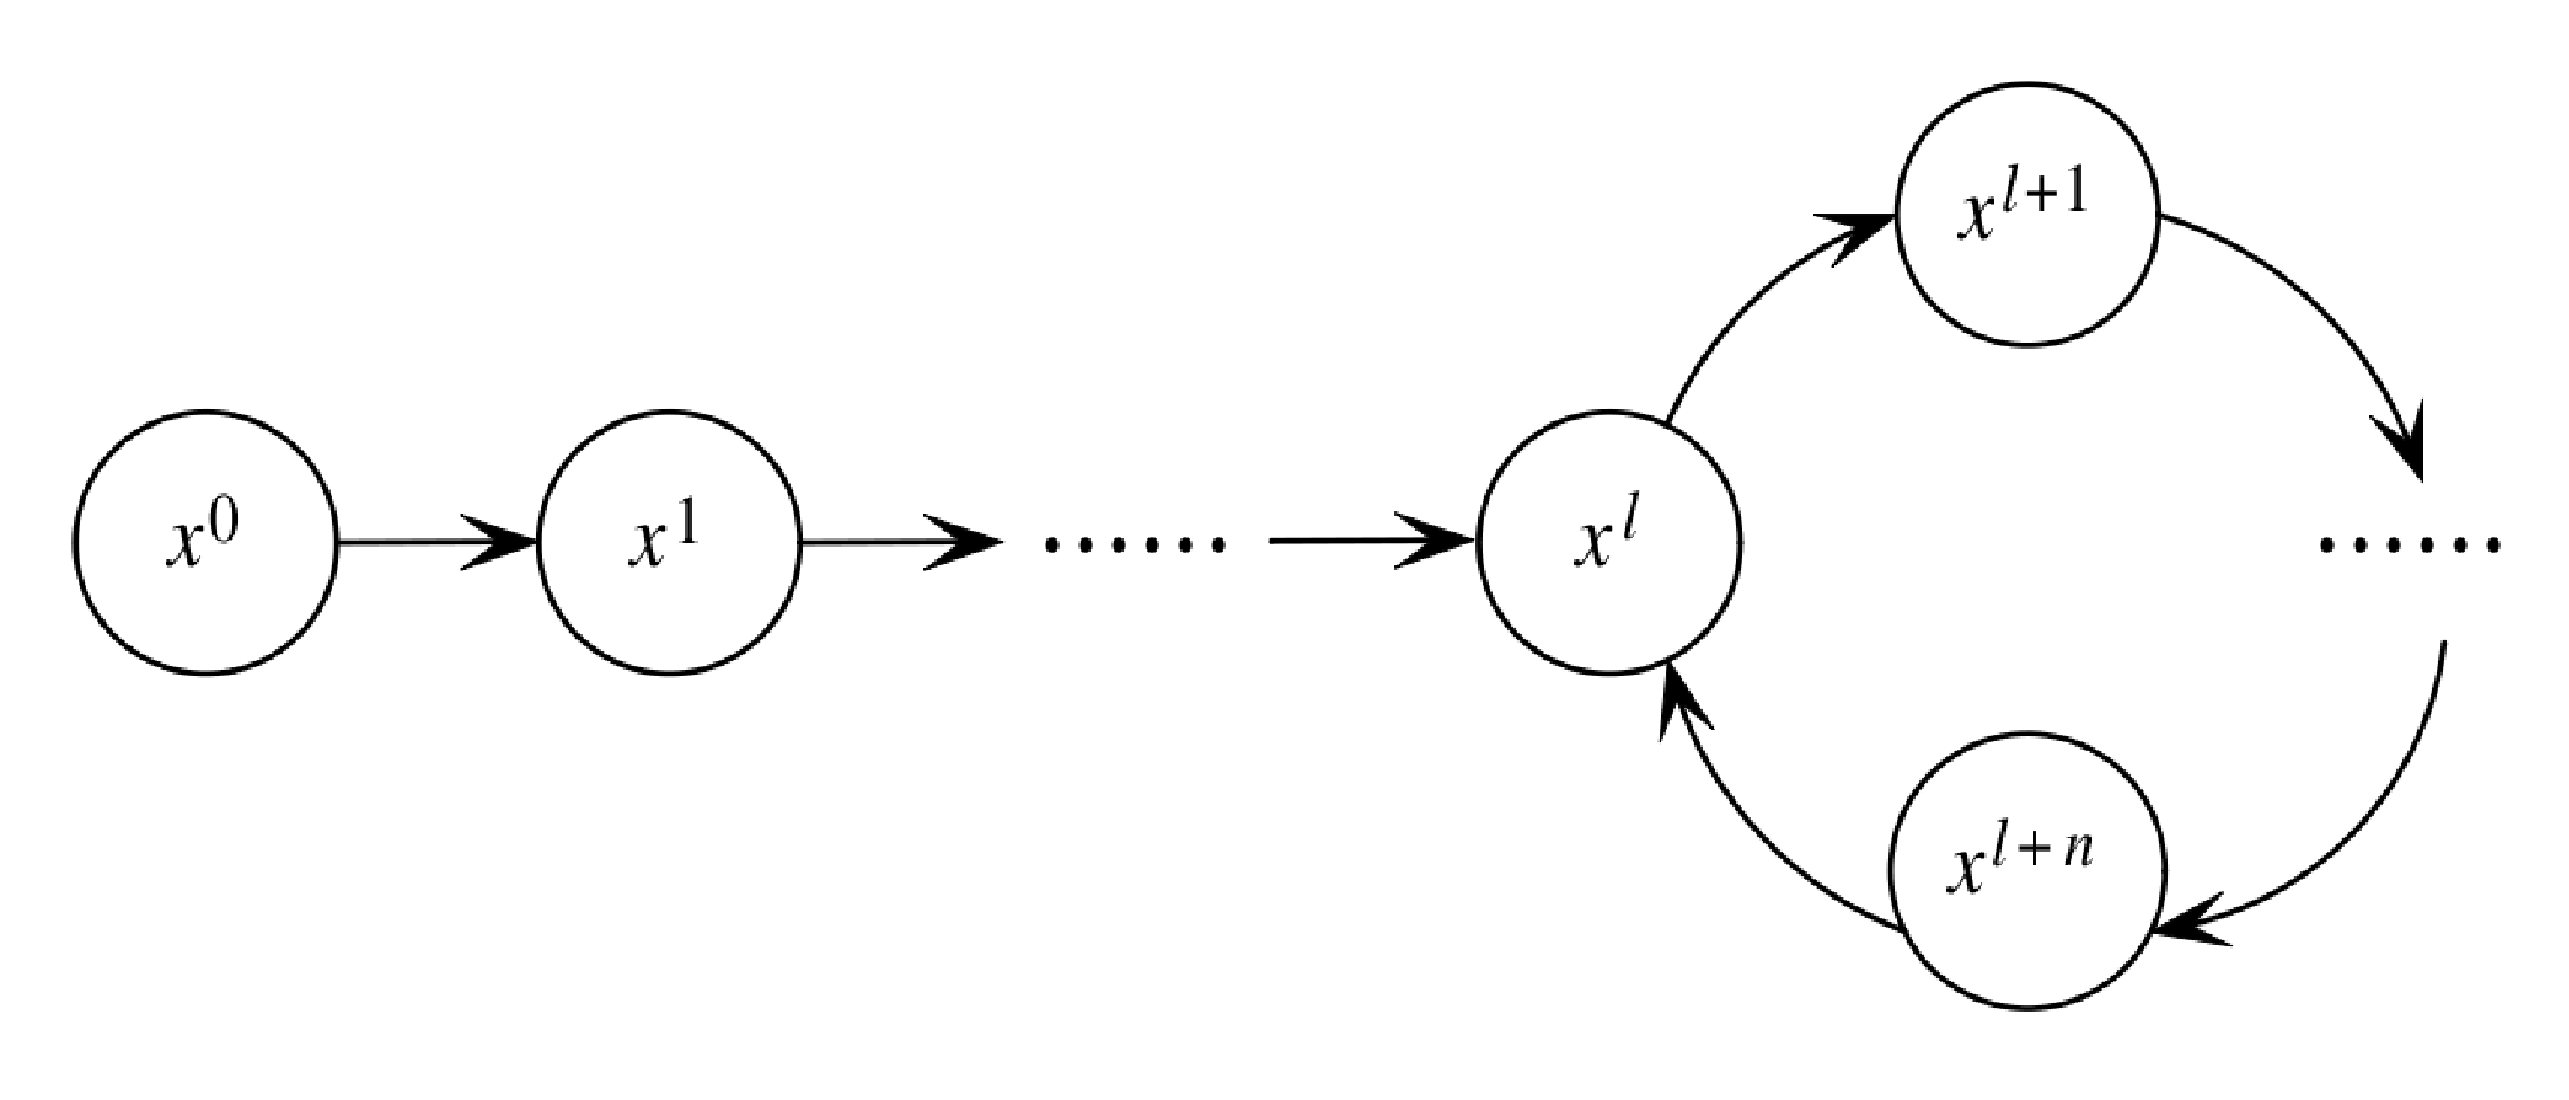
\includegraphics[scale=0.20]{pseudo_orbit.eps}
\caption{A pseudo orbit of a digital chaotic system}
\label{A pseudo orbit of a digital chaotic system}
\end{figure}


\begin{definition}%\cite{bahi102008}
A sequence $x = (x^{ 1} , ..., x^{n} )$ is said to be cyclic if a subset of successive terms is repeated from a given rank, until the end of $x$.
\end{definition}

This generator based on discrete chaotic iterations generated by two pseudorandom sequences ($m$ and $w$) has a long cycle length. If the cycle period of $m$ and $w$ are respectivelly $n_{m}$ and $n_{w}$, then in an ideal situation, the cycle period of the novel sequence is $n_{m} \times n_{w}\times 2$ (because $\bar{\bar{x}}=x$). Table \ref{The ideal cycle period} gives the ideal cycle period of various generators.

\begin{itemize}
\item $m$ ($n_{m}=2$): 12121212121212121212121212...

\item $w$ ($n_{w}=4$): 1 23 4 12 3 41 2 34 1 23 4 12 3 41 2 34 1 23 4...

\item $x$ ($n_{x}=2 \times 4 \times 2=16$): 0000(0) 1000(8) 1110(14) 1111(15) 0011(3) 0001(1) 1000(8) 1100(12) 1111(15) 0111(7) 0001(1) 0000(0) 1100(12) 1110(14) 0111(7) 0011(3) 0000(0) 1000(8) 1110(14) 1111(15) 0011(3) 0001(1) 1000(8) 1100(12) 1111(15) 0111(7) 0001(1) 0000(0) 1100(12) 1110(14) 0111(7) 0011(3)...

\end{itemize}


\begin{table}
\renewcommand{\arraystretch}{1.3}
\caption{Ideal cycle period}
\label{The ideal cycle period}
\centering
% \begin{tiny}
\begin{tabular}{|c|c|c|}\toprule\hline
\multicolumn{2}{|c|}{\textbf{PRNG}}&\textbf{Ideal cycle period}\\\hline
\multicolumn{2}{|c|}{\textbf{Logistic map}}& $\infty$\\\hline
\multicolumn{2}{|c|}{\textbf{XORshift}}&$2^{32}-1$ \\\hline
\multicolumn{2}{|c|}{\textbf{ISAAC}}& $2^{8295}$\\\hline
\multirow{4}*{\textbf{Version 1 CI algorithms}}&\textbf{Logistic map 1+Logistic map 2}&$\infty$\\\cline{2-3}
&\textbf{XORshift+XORshift}&$2^{65}$\\\cline{2-3}
&\textbf{XORshift+ISAAC}&$2^{8328}$\\\cline{2-3}
&\textbf{ISAAC+ISAAC}&$2^{16591}$\\\hline
\bottomrule
\end{tabular}
% \end{tiny}
\end{table}

\subsection{Security Analysis}
\label{Security Analysis Version 1 CI}
In this section the concatenation of two strings $u$ and $v$ is classically denoted by $uv$.
In a cryptographic context, a pseudo random generator is a deterministic algorithm $G$ transforming 
strings into strings and such that, for any seed 
$s$ of length m, $G(s)$ (the output of $G$ on the input $s$) has size $l_G(m)$ with $l_G(m) > m$. The notion of secure 
PRNGs can now be defined as follows.
\subsubsection{Algorithm expression conversion}
For the convenience of security analysis, Version 1 CI Algorithm \ref{Chaotic iteration} is converted as 
Equation~\ref{Version 1 CI Eq}, internal state is $x$, $S$ and $T$ are those computed by PRNG1 and PRNG2, 
each round, $x^{n-1}$ is updated to be $x^n$. 

\begin{equation}
\left\{
\begin{array}{l}
x^0 \in \llbracket 0, 2^\mathsf{N}-1 \rrbracket, S \in \llbracket 0, 2^\mathsf{N}-1 \rrbracket^\mathds{N}, T \in \llbracket 0, 2^\mathsf{N}-1 \rrbracket^\mathds{N}\\
C = S^n \& 1 + 3*N\\
w^0 = {T}^m~mod~N, w^1 = {T}^{m+1} \& 3, ... w^{C-1} = {T}^{m+C-1} \& 3\\ 
d^n = (1 \ll w^0) \oplus (1\ll w^1) \oplus ... (1 \ll w^{C-1})\\
\forall n \in \mathds{N}^*, x^n = x^{n-1} \oplus d^n,
\end{array}
\right.
\label{Version 1 CI Eq}
\end{equation}


\subsubsection{Proof}
\begin{definition}
\label{CSPRNG}
A cryptographic PRNG $G$ is secure if for any probabilistic polynomial time algorithm D, for any positive polynomial p, 
and for all sufficiently large m's,  
\begin{equation}
|Pr[D(G(U_m))=1]-Pr[D(U_{l_G(m)})=1]<\frac{1}{p(m)},
\end{equation}
where $U_r$ is the uniform distribution over ${0, 1}^r$ and the probabilities are taken over $U_m$, 
$U_{l_G(m)}$ as well as over the internal coin tosses of $D$.
\end{definition}

Intuitively, it means that there is no polynomial time algorithm that can distinguish a perfect uniform 
random generator from $G$ with a non negligible probability. Note that it is quite easily possible to change 
the function $l$ into any polynomial function $l'$ satisfying $l'(m)>m$.

The generation schema developed in Algorithm~\ref{Version 1 CI Eq} is based on $2$ pseudo random generators. Let $H$ 
be the ``PRNG1'' and $I$ be the ``PRNG2''. 
We may assume, without loss of generality, that for any string $S_0$ of size $L$,
the size of $H(S_0)$ is $kL$,  then for any string $T_0$ of size $M$, it has $I(T_0)$ with $kN$, with $k > 2$. 
It means that $l_H(N) = kL$ and $l_I(N) = kM$. Let $S_1,...,S_k$ be the string of length $L$ such that 
$H(S_0) = S_1 ... S_k$ and $T_1,...,T_k$ be the string of length
$M$ that $H(S_0) = T_1 ... T_k$ ($H(S_0)$ and $I(T_0)$ are the concatenations of $S_i$'s and $T_i$'s).
The cryptographic PRNG $X$ defined in Algorithm~\ref{Version 1 CI Eq} is algorithm mapping any string of length 
$L+M+N~ x_0S_0T_0$ into the string $x_0 \oplus d^1, 
x_0 \oplus d^1 \oplus d^2,... 
(x_0 \bigoplus^{i=k}_{i=0}d^i)$ (Equation~\ref{Version 1 CI Eq}).
One in particular has $l_X(L+M+N) = kN = l_H(N)$ and $k > M+L+N$.
We announce that if one PRNG of $H$ is secure, then the new one from Equation \ref{Version 1 CI Eq} 
is secure too.

\begin{proposition}
\label{cryptopreuve}
If one of $H$ is a secure cryptographic PRNG, then $X$ is a secure cryptographic
PRNG too.
\end{proposition}

\begin{proof}
The proposition is proven by contraposition. Assume that $X$ is not
secure. By Definition, there exists a polynomial time probabilistic
algorithm $D$, a positive polynomial $p$, such that for all $k_0$ there exists
$L+M+N\geq {k_0}$ satisfying 
$$| \mathrm{Pr}[D(X(U_{L+M+N}))=1]-\mathrm{Pr}[D(U_{kN}=1]|\geq \frac{1}{p(L+M+N)}.$$

Define there is a $w$ of size $kL$.
\begin{enumerate}
 \item Decompose $w$ into $w = w_1...w_k$.
 \item Pick a string $y$ of size $N$ uniformly at random.
 \item Pick a string of size $(3kN + \sum_{j=1}^{j=k}(w_j\&1)) M$: $u$.
 \item Decompose $u$ into $u = u_1...u_{3kN + \sum_{j=1}^{j=k}(w_j\&1)}$.
 \item Define $t_i = (\bigoplus_{l=3N(i-1)+(\sum_{l=1}^{l=i-1}(w_j\&1))+1}^
 {j=3N(i)+(\sum_{j=1}^{j=i}(w_j\&1))}(1<<u_l))$.
 \item Compute $z = (y\oplus t_1) (y\oplus t_1 \oplus t_2) ... (y\bigoplus_{i=1}^{i=k}(t_i))$.
 \item Return $D(z)$.
\end{enumerate}


On one hand, consider for each $y\in \mathbb{B}^{kN}$ the function $\varphi_{y}$
from $\mathbb{B}^{kN}$ into $\mathbb{B}^{kN}$ mapping $t=t_1\ldots t_k$
(each $t_i$ has length $N$) to 
$(y\oplus t_1 )(y\oplus t_1\oplus t_2)\ldots (y
  \bigoplus_{i=1}^{i=k} t_i)$. 
 On the other hand, treat each $u_l \in \mathbb{B}^{(3Nk + \sum_{j=0}^{j=k}(w_j\&1)) M}$ the function $\phi_{u}$
 from $\mathbb{B}^{(3kN + \sum_{j=0}^{j=k}(w_i\&1)) M}$ into $mathbb{B}^{kN}$ mapping $w = w_1 \ldots w_k$ (each 
 $w_i$ has length $L$) to 
 $(\bigoplus_{l=1}^{l=3N+(w_1\&1)}(1<<u_l)) ((\bigoplus_{l=1+3N+(w_1\&1)}^{l=6N+(w_1\&1)+(w_1\&1)}(1<<u_l)) \ldots 
 (\bigoplus_{l=3N(k-1)+\sum_{j=1}^{j=k-1}(w_j\&1)}^{l=3Nk+\sum_{j=1}^{j=k}(w_j\&1)}(1<<u_l)$
 By construction, one has for every $w$,
  
\begin{equation}\label{PCH-1}
D^\prime(w)=D(\varphi_y(\phi_u(w))),
\end{equation}

Therefore, and using (\ref{PCH-1}),
one has
$\mathrm{Pr}[D^\prime(U_{kL})=1]=\mathrm{Pr}[D(\varphi_y(\phi_u(U_{kL})))=1]$ and,
therefore, 
\begin{equation}\label{PCH-2}
\mathrm{Pr}[D^\prime(U_{kL})=1]=\mathrm{Pr}[D(U_{kN})=1].
\end{equation}

Now, using (\ref{PCH-1}) again, one has  for every $x$,
\begin{equation}\label{PCH-3}
\mathrm{Pr}[D^\prime(U_{H(x)})=1]=\mathrm{Pr}[D(\varphi_y(\phi_u(U_{H(x)})))=1] 
\end{equation}

since where $y$ and $u_j$ are randomly generated. \\
By construction, $\varphi_y(\phi_u(x))=X(yu_1w)$, hence 

\begin{equation}\label{PCH-4}
\mathrm{Pr}[D^\prime(H(U_{kL}))=1]=\mathrm{Pr}[D(X(U_{N+M+L}))=1]
\end{equation}

Compute the difference of Equation (\ref{PCH-4}) and (\ref{PCH-3}), one can deduce that
there exists a polynomial time probabilistic
algorithm $D^\prime$, a positive polynomial $p$, such that for all $k_0$ there exists
$L+M+N\geq {k_0}$ satisfying 
$$| \mathrm{Pr}[D^\prime(H(U_{KL}))=1]-\mathrm{Pr}[D(U_{kL})=1]|\geq \frac{1}{p(L+M+N)},$$
proving that $H$ is not secure, which is a contradiction to the first place that one 
of them is cryptographic secure. 
\end{proof}

\subsection{An Efficient, Cryptographically Secure, PRNG Based On Version 1 CI}
In Table~\ref{Version 1 CI cs}, an efficient, based on Version 1 CI, good random quality, and cryptographically secure 
PRNG algorithm is given.

\begin{table}
\centering
\begin{tabular}{|l|l|}
\hline
~\textbf{Input}: $x$ (a 12-bit word)\\
\hline
~\textbf{Output}: $r$ (a 12-bit word)\\
\hline
~$x1 \leftarrow xorshift1();$\\
~$x2 \leftarrow xorshift2();$\\
~$x3 \leftarrow xorshift3();$\\
~$t \leftarrow bbs();$\\
~$t1 \leftarrow t \& 1;$\\
~$t2 \leftarrow t \& 2;$\\
~$t3 \leftarrow t \& 4;$\\
~$w1 \leftarrow 0;$\\
~$w2 \leftarrow 0;$\\
~$w3 \leftarrow 0;$\\
~$\textbf{While}~ i = 1 ... 12$ \\
~$w1 \leftarrow (w1 \oplus (1 \ll ((x1 \gg (i\times 2))\&3)));$\\
~$w2 \leftarrow (w2 \oplus (1 \ll ((x2 \gg (i\times 2))\&3)));$\\
~$w3 \leftarrow (w3 \oplus (1 \ll ((x3 \gg (i\times 2))\&3)));$\\
~$\textbf{EndWhile}$\\
~$\textbf{if}~(t1 \neq 0)~\textbf{then}~w1 \leftarrow (w1 \oplus (1 \ll ((x1 \gg 26)\&3)));$ \\
~$\textbf{if}~(t2 \neq 0)~\textbf{then}~w2 \leftarrow (w2 \oplus (1 \ll ((x2 \gg 26)\&3)));$ \\
~$\textbf{if}~(t3 \neq 0)~\textbf{then}~w3 \leftarrow (w3 \oplus (1 \ll ((x3 \gg 26)\&3)));$ \\
~$x \leftarrow x \oplus w1 \oplus (w2 \ll 4) \oplus (w3 \ll 8);$\\
~$r \leftarrow x;$\\
~$\textbf{return} ~r;$\\
\hline
~\textbf{An arbitrary round of the algorithm}~\\
\hline
\end{tabular}
\caption{An Efficient, Cryptographically Secure, PRNG Based On Version 1 CI}
\label{Version 1 CI cs}
\end{table}

The internal state $x$ is defined as size of $12$ bits, three $32$-bit
XORshift PRNGs ($xorshift1(), xorshift2(), xorshift3()$) are applied, 
each of them is split to $16$ $2$-bit binary blocks (value is between 
$0$ to $3$), then the $3$ LSBs (least significant bits) of the output 
from BBS $bbs()$ are decide $12$ or $13$ these blocks used to update the 
state. According to Section~\ref{Security Analysis Version 1 CI}, this 
generator based on Version 1 CI can turn to be cryptographically secure if 
its $I$ used is cryptographically secure, here $I$ is chosen as BBS PRNG, 
which is believed to be the most secure PRNG method available~\cite{vmd}, 
the $t$ computed by BBS $bbs()$ is based on $32$ bit $m$ (Equation~\ref
{BBS Eq}), the $log(log(m))$ LSBs of $t$ can be treated as secure, hence, 
here $3$LSBs chosen is qualified.

\section{Version 2 CIPRNG Algorithm}
\subsection{Presentation}
The CI generator (generator based on chaotic iterations) is designed by the following process.
First of all, some chaotic iterations have to be done to generate a sequence 
$\left(x^n\right)_{n\in\mathds{N}} \in \left(\mathds{B}^\mathsf{N}\right)^\mathds{N}$ 
($\mathsf{N} \in \mathds{N}^*, \mathsf{N} \geqslant 2$, $N$ is not necessarily equal to 32) 
of boolean vectors, which are the successive states of the iterated system. Some of these vectors 
will be randomly extracted and our pseudo-random bit flow will be constituted by their components. 
Such chaotic iterations are realized as follows. 
Initial state $x^0 \in \mathds{B}^\mathsf{N}$ is a boolean vector taken as a 
seed (see Section~\ref{algo seed}) and chaotic strategy $\left(S^n\right)_{n\in\mathds{N}}\in 
\llbracket 1, \mathsf{N} \rrbracket^\mathds{N}$ is
an irregular decimation of a random number sequence (Section~\ref{Chaotic strategy}). The iterate function $f$ is
the vectorial boolean negation:
$$f_0:(x_1,...,x_\mathsf{N}) \in \mathds{B}^\mathsf{N} \longmapsto 
(\overline{x_1},...,\overline{x_\mathsf{N}}) \in \mathds{B}^\mathsf{N}.$$
At each iteration, only the $S^i$-th component of state $x^n$ is updated, 
as follows: $x_i^n = x_i^{n-1}$ if $i \neq S^i$, else $x_i^n = \overline{x_i^{n-1}}$.
Finally, some $x^n$ are selected
by a sequence $m^n$ as the pseudo-random bit sequence of our generator.
$(m^n)_{n \in \mathds{N}} \in \mathcal{M}^\mathds{N}$ is computed from 
a PRNG, such as XORshift sequence $(y^n)_{n \in \mathds{N}} \in \llbracket 0, 
2^{32}-1 \rrbracket$ (see Section~\ref{algo m}). So, the
generator returns the following values:\newline
\begin{small}
Bits:$$x_1^{m_0}x_2^{m_0}x_3^{m_0}\hdots x_\mathsf{N}^{m_0}x_1^{m_0+m_1}x_2^{m_0+m_1}\hdots x_\mathsf{N}^{m_0+m_1} x_1^{m_0+m_1+m_2}\hdots$$
or States:$$x^{m_0}x^{m_0+m_1}x^{m_0+m_1+m_2}\hdots$$
\end{small}


\subsection{The seed}
\label{algo seed}
The unpredictability of random sequences is established using
a random seed that is obtained by a physical source like timings of keystrokes.
Without the seed, the attacker must not be able to make any predictions about
the output bits, even when all details of the generator are known~\cite{Turan2008}.

The initial state of the system $x^0$ and the first term $y^0$ of the input PRNG are seeded either by
the current time in seconds since the Epoch, or by a number that the user inputs.
Different ways are possible. For example, let us denote by $t$ the decimal part of the current
time. So $x^0$ can be $t \text{ (mod $2^N$)}$ written in binary digits and $y^0 = t$.

\subsection{Sequence $m$ of returned states}
\label{algo m}
The output of the sequence $(y^n)$ is uniform in $\llbracket 0, 2^{32}-1 \rrbracket$. However, we do not want the output of $(m^n)$ to be uniform in $\llbracket 0, N \rrbracket$, because in this case, the returns of our generator will not be uniform in $\llbracket 0, 2^{N}-1 \rrbracket$, as it is illustrated in the following example. Let us suppose that $x^0=(0,0,0)$. Then $m^0 \in \llbracket 0, 3 \rrbracket$.
\begin{itemize}
\item If $m^0=0$, then no bit will change between the first and the second output of our new CI PRNG. Thus $x^1 = (0,0,0)$.
\item If $m^0=1$, then exactly one bit will change, which leads to three possible values for $x^1$, namely $(1,0,0)$, $(0,1,0)$, and $(0,0,1)$.
\item \emph{etc.}
\end{itemize}
As each value in $\llbracket 0, 2^3-1 \rrbracket$ must be returned with the same probability, then the values $(0,0,0)$, $(1,0,0)$, $(0,1,0)$, and $(0,0,1)$ must occur for $x^1$ with the same probability. Finally we see that, in this example, $m^0=1$ must be three times probable as $m^0=0$.
This leads to the following general definition for the probability of $m=i$:
\begin{equation}
P(m^n=i)=\frac{C^i_N}{2^N}
\end{equation}

Then, here is an example for the $(m^n)$ sequence with a selector function $g_1$
\begin{equation}
\label{v2_g1}
m^n = g_1(y^n)=
\left\{
\begin{array}{l}
0 \text{ if }0 \leqslant\frac{y^n}{2^{32}}<\frac{C^0_N}{2^N},\\
1 \text{ if }\frac{C^0_N}{2^N} \leqslant\frac{y^n}{2^{32}}<\sum_{i=0}^1\frac{C^i_N}{2^N},\\
2 \text{ if }\sum_{i=0}^1\frac{C^i_N}{2^N} \leqslant\frac{y^n}{2^{32}}<\sum_{i=0}^2\frac{C^i_N}{2^N},\\
\vdots~~~~~ ~~\vdots~~~ ~~~~\\
N \text{ if }\sum_{i=0}^{N-1}\frac{C^i_N}{2^N} \leqslant\frac{y^n}{2^{32}}<1.\\
\end{array}
\right.
\end{equation}

Let us notice, to conclude this subsection, that our new CI PRNG can use any reasonable function as selector. 
In this paper, $g_1()$ and $g_2()$ are adopted for demonstration purposes, where:
\begin{equation}
\label{v2_g2}
m^n = g_2(y^n)=
\left\{
\begin{array}{l}
N \text{ if }0 \leqslant\frac{y^n}{2^{32}}<\frac{C^0_N}{2^N},\\
N-1 \text{ if }\frac{C^0_N}{2^N} \leqslant\frac{y^n}{2^{32}}<\sum_{i=0}^1\frac{C^i_N}{2^N},\\
N-2 \text{ if }\sum_{i=0}^1\frac{C^i_N}{2^N} \leqslant\frac{y^n}{2^{32}}<\sum_{i=0}^2\frac{C^i_N}{2^N},\\
\vdots~~~~~ ~~\vdots~~~ ~~~~\\
0 \text{ if }\sum_{i=0}^{N-1}\frac{C^i_N}{2^N} \leqslant\frac{y^n}{2^{32}}<1.\\
\end{array}
\right.
\end{equation}

In this thesis, $g_1()$ is the selector function unless noted otherwise. And we will show later that both of $g_1()$ and $g_2()$ can pass all of the performed tests. 

\begin{figure}
\centering
\subfigure [The histogram of adjacent output distribution $m^n = g_1(y^n)$]{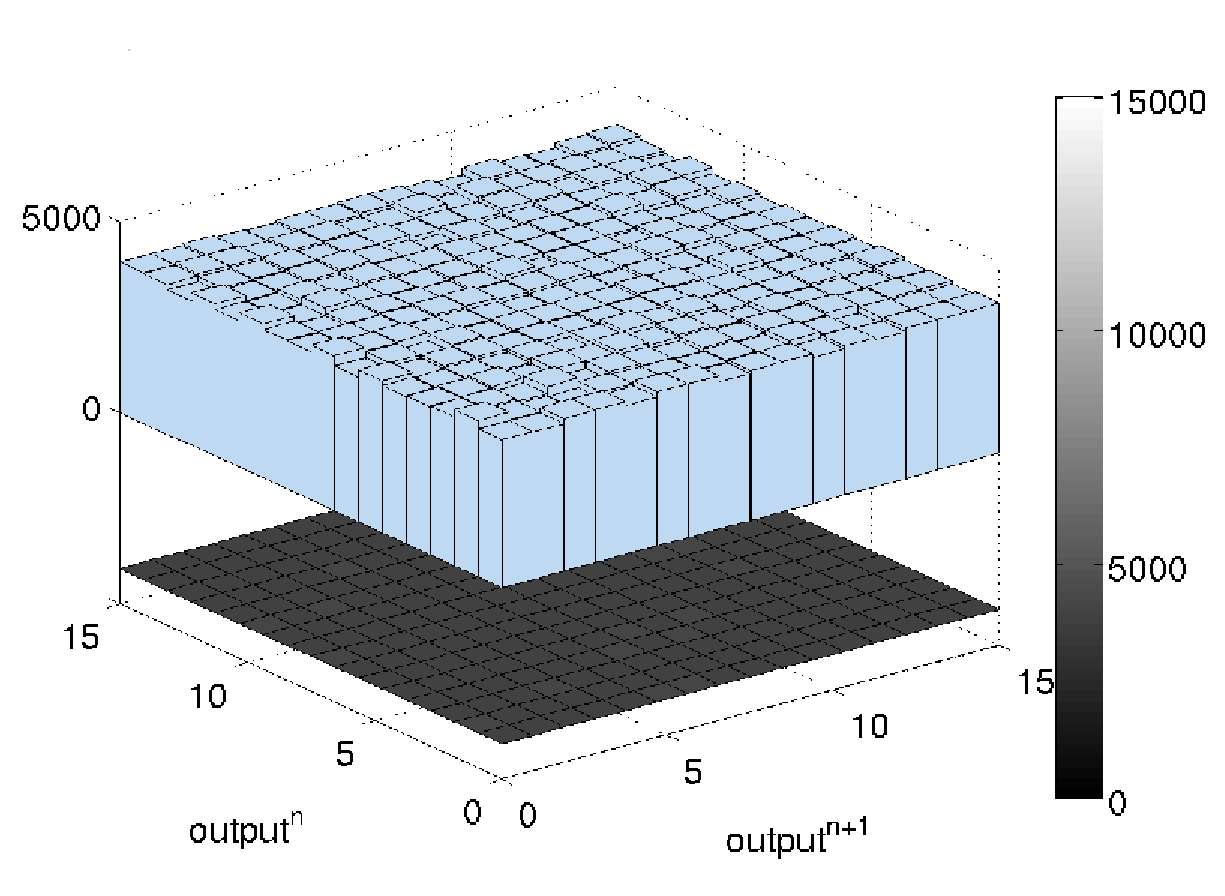
\includegraphics[scale=0.4]{fy.eps}
\label{Histogram1}} \hspace{0.4cm}
\subfigure [The histogram of adjacent output distribution $m^n = g_2(y^n)$]{\includegraphics[scale=0.3]{f2y.eps}
\label{Histogram2}} \hspace{0.4cm}
\subfigure [The histogram of adjacent output distribution $m^n = y^n ~ mod ~ 4$]{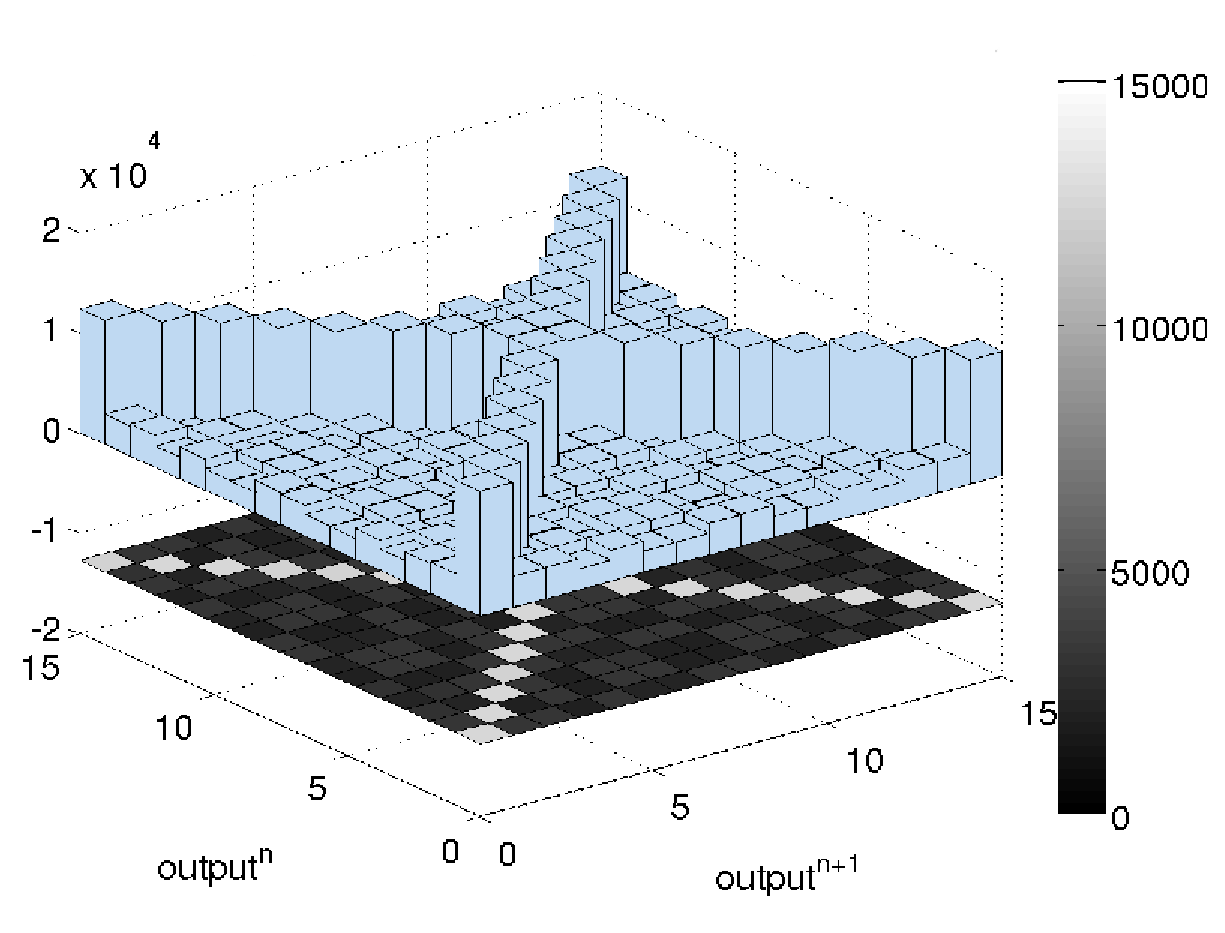
\includegraphics[scale=0.4]{y.eps}%
\label{Histogram3}} \hspace{0.4cm}
\caption{Histogram and intensity maps}
\label{Histogram and intensity map1}
\end{figure}

In order to evaluate our proposed method and compare its statistical properties with various other methods, the density histogram and intensity map of adjacent output have been computed. The length of $x$ is $N = 4$ bits, and the initial conditions and control
parameters are the same. A large number of
sampled values are simulated ($10^6$ samples). 
Figure~\ref{Histogram1} and Figure~\ref{Histogram2} shows the intensity map for $m^n=g_1(y^n)$ and $m^n=g_2(y^n)$.
In order to appear random, the histogram should be uniformly distributed in all areas. 
It can be observed that uniform histograms and flat color intensity maps are obtained when using our schemes. 
Another illustration of this fact is given by Figure~\ref{Histogram3}, whereas its uniformity is further justified by the tests presented in Section \ref{Test for Version 2 CI}.


\subsection{Chaotic strategy}
\label{Chaotic strategy}
The chaotic strategy $(S^k) \in \llbracket 1, N \rrbracket^\mathds{N}$ is generated from a second XORshift sequence $(b^k) \in \llbracket 1, N \rrbracket^\mathds{N}$. The only difference between the sequences $S$ and $b$ is that some terms of $b$ are discarded, in such a way that $\forall k \in \mathds{N}, (S^{M^k}, S^{M^k+1}, \hdots, S^{M^{k+1}-1})$ does not contain any given integer twice, where $M^k = \sum_{i=0}^k m^i$. Therefore, no bit will change more than once between two successive outputs of our PRNG, increasing the speed of the former generator by doing so. $S$ is said to be ``an irregular decimation'' of $b$. This decimation can be obtained by the following process.

Let $(d^1,d^2,\dots,d^N)\in \{0,1\}^N$ be a mark sequence, such that whenever $\sum_{i=1}^N d^i = m^k$,
then $\forall i, d_i=0$ ($\forall k$, the sequence is reset when $d$ contains $m^k$ times the number 1). This mark sequence will control the XORshift sequence $b$ as follows:
\begin{itemize}
\item if $d^{b^j} \neq 1$, then $S^k=b^j$, $d^{b^j} = 1$, and $k = k+1$,
\item if $d^{b^j}=1$, then $b^j$ is discarded.
\end{itemize}
For example, if $b = 142\underline{2}334 1421\underline{1}\underline{2}\underline{2}34...$ and $m = 4341...$, then $S=1423~341~4123~4...$ However, if we do not use the mark sequence, then one position may change more than once and the balance property will not be checked, due to the fact that $\bar{\bar{x}}=x$. As an example, for $b$ and $m$ as in the previous example, $S=1422~334~1421~1...$ and $S=14~4~42~1...$ lead to the same output (because switching the same bit twice leads to the same state).

 
To check the balance property, a set of 500
sequences are generated with and without decimation, each
sequence containing $10^6$ bits. Figure~\ref{nmark} shows the
percentages of differences between zeros and ones, and presents a better balance property for the sequences with decimation. This claim will be verified in the tests section (Section \ref{Results of NISTfor new CI}). 


Another example is given in Table~\ref{table application example}, in which $r$ means ``reset'' and the integers which are underlined in sequence $b$ are discarded.





\begin{figure}
\centering
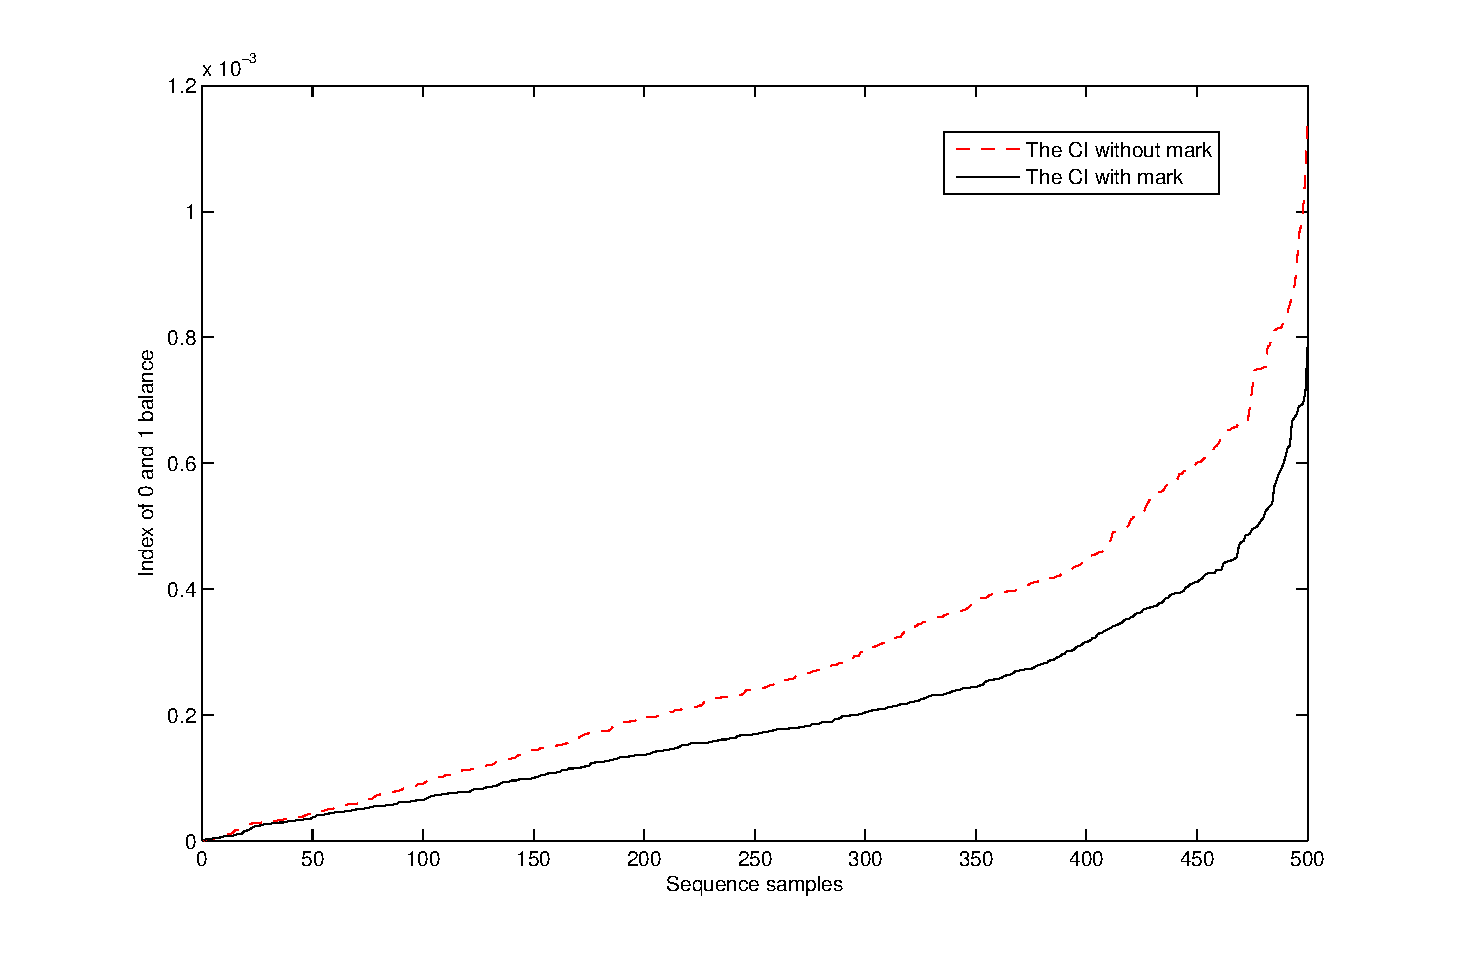
\includegraphics[width=3.85in]{nmark.eps}
\DeclareGraphicsExtensions.
\caption{Balance property}
\label{nmark}
\end{figure}

\subsection{Version 2 CI Algorithm}

The basic design procedure of the novel generator is summed up in Algorithm~\ref{Chaotic iteration1}.
The internal state is $x$, the output state is $r$. $a$ and $b$ are those computed by the two input
PRNGs. The value $g_1(a)$ is an integer, defined as in Equation~\ref{v2_g1}. Lastly, $\mathsf{N}$ is a constant 
defined by the user.
\begin{algorithm}
\textbf{Input:} the internal state $x$ ($\mathsf{N}$ bits)\\
\textbf{Output:} a state $r$ of $\mathsf{N}$ bits
\begin{algorithmic}[1]
\FOR{$i=0,\dots,N$}
{
\STATE$d_i\leftarrow{0}$\;
}
\ENDFOR
\STATE$a\leftarrow{PRNG1()}$\;
\STATE$m\leftarrow{f(a)}$\;
\STATE$k\leftarrow{m}$\;
\WHILE{$i=0,\dots,k$}

\STATE$b\leftarrow{PRNG2()~mod~\mathsf{N}}$\;
\STATE$S\leftarrow{b}$\;
    \IF{$d_S=0$}
    {
\STATE      $x_S\leftarrow{ \overline{x_S}}$\;
\STATE      $d_S\leftarrow{1}$\;
    
    }
    \ELSIF{$d_S=1$}
    {
\STATE      $k\leftarrow{ k+1}$\;
    }\ENDIF
\ENDWHILE
$r\leftarrow{x}$\;
return $r$\;
\medskip
\caption{An arbitrary round of the Version 2 CI generator}
\label{Chaotic iteration1}
\end{algorithmic}
\end{algorithm}


As a comparison, the basic design procedure of the old generator 
is recalled in Algorithm~\ref{Chaotic iteration2} ($a$ and $b$ are computed by two input PRNGs, 
$\mathsf{N}$ and $c\geqslant 3\mathsf{N}$ are constants defined by the user). 
See Subsection~\ref{Version 1 CI algorithms and examples} for further information.


\begin{algorithm}
\textbf{Input:} the internal state $x$ (an array of $\mathsf{N}$ 1-bit words)\\
\textbf{Output:} an array $r$ of $\mathsf{N}$ 1-bit words
\begin{algorithmic}[1]

\STATE$a\leftarrow{PRNG1()}$;
\STATE$m\leftarrow{a~mod~2+c}$;
\WHILE{$i=0,\dots,m$}
\STATE$b\leftarrow{PRNG2()}$;
\STATE$S\leftarrow{b~mod~\mathsf{N}}$;
\STATE$x_S\leftarrow{ \overline{x_S}}$;
\ENDWHILE
\STATE$r\leftarrow{x}$;
\STATE return $r$;
\medskip
\caption{An arbitrary round of the old CI generator}
\label{Chaotic iteration2}
\end{algorithmic}
\end{algorithm}


\subsection{Illustrative Example of Version 2 CI (XORshift, XORshift)}

In this example, $\mathsf{N} = 4$ is chosen for easy understanding and the input PRNG is XORshift PRNG.
As stated before, the initial state of the system $x^0$ can be seeded by the decimal part $t$ of the current time.
For example, if the current time in seconds since the Epoch is 1237632934.484088,
so $t = 484088$, then $x^0 = t \text{ ($mod$ 16)}$ in binary digits, \emph{i.e.}, $x^0 = ( 0, 1, 0, 0)$.

To compute $m$ sequence, Equation~\ref{v2_g1} can be adapted to this example as follows:
\begin{equation}
\label{m1 fuction}
m^n=g_1(y^n)=
\left\{
\begin{array}{llccccc}
0 & \text{ if }&0 &\leqslant&\frac{y^n}{2^{32}}&<&\frac{1}{16},\\
1 & \text{ if }&\frac{1}{16} &\leqslant&\frac{y^n}{2^{32}}&<&\frac{5}{16} ,\\
2 & \text{ if }&\frac{5}{16} &\leqslant&\frac{y^n}{2^{32}}&<&\frac{11}{16},\\
3 & \text{ if }&\frac{11}{16} &\leqslant&\frac{y^n}{2^{32}}&<&\frac{15}{16},\\
4 & \text{ if }&\frac{15}{16} &\leqslant&\frac{y^n}{2^{32}}&<&1,\\
\end{array}
\right.
\end{equation}

\noindent where $y$ is generated by XORshift seeded with the current time. 
We can see that the probabilities of occurrences of $m=0$, $m=1$, $m=2$, $m=3$, $m=4$, 
are $\frac{1}{16}$, $\frac{4}{16}$, $\frac{6}{16}$, $\frac{4}{16}$, $\frac{1}{16}$, respectively. 
This $m$ determines what will be the next output $x$. For instance,
\begin{itemize}
\item If $m=0$, the following $x$ will be $( 0, 1, 0, 0)$.
\item If $m=1$, the following $x$ can be $( 1, 1, 0, 0)$, $( 0, 0, 0, 0)$, $( 0, 1, 1, 0)$, or $( 0, 1, 0, 1)$.
\item If $m=2$, the following $x$ can be $( 1, 0, 0, 0)$, $( 1, 1, 1, 0)$, $( 1, 1, 0, 1)$, $( 0, 0, 1, 0)$, $( 0, 0, 0, 1)$, or $( 0, 1, 1, 1)$.
\item If $m=3$, the following $x$ can be $( 0, 0, 1, 1)$, $( 1, 1, 1, 1)$, $( 1, 0, 0, 1)$, or $( 1, 0, 1, 0)$.
\item If $m=4$, the following $x$ will be $( 1, 0, 1, 1)$.
\end{itemize}

In this simulation, $m = 0, 4, 2, 2, 3, 4, 1, 1, 2, 3, 0, 1, 4,...$ Additionally, 
$b$ is computed with a XORshift generator too, but with another seed. We have found 
$b = 1, 4, 2, 2, 3, 3, 4, 1, 1, 4, 3, 2, 1,...$

Chaotic iterations are made with initial state $x^0$, vectorial logical negation $f_0$, and
strategy $S$. The result is presented in Table~\ref{table application example}. Let us 
recall that sequence $m$ gives the states $x^n$ to return, which are here $x^0, x^{0+4}, 
x^{0+4+2}, \hdots$ So, in this example, the output of the generator is: 10100111101111110011... or 4,4,11,8,1...




\begin{table*}[!t]
%\renewcommand{\arraystretch}{1.3}
\centering
\begin{tabular}{|c|c@{}c|c@{}c@{}c@{}c@{}c@{}c|c@{}c@{}c|c@{}c@{}c@{}c|}
\hline
$m$ &0 & &4 & & & & & &2& &&2&&  &  \\ \hline
$k$ &0 & &4 & & &$+1$ & & &2& &&2&$+1$&  &  \\ \hline
$b$  &  & &1 &4&2&\underline{2}       &3& &3&4&&1&\underline{1}      &4&\\ \hline
$d$  &r  & &r~$\left(\begin{array}{c}1\\0\\0\\0\end{array}\right)$ & $\left(\begin{array}{c}1\\0\\0\\1\end{array}\right)$ & $\left(\begin{array}{c}1\\1\\0\\1\end{array}\right)$ & & $\left(\begin{array}{c}1\\1\\1\\1\end{array}\right)$ && r~$\left(\begin{array}{c}0\\0\\1\\0\end{array}\right)$ &$\left(\begin{array}{c}0\\0\\1\\1\end{array}\right)$ &&r~$\left(\begin{array}{c}1\\0\\0\\0\end{array}\right)$ & &$\left(\begin{array}{c}1\\0\\0\\1\end{array}\right)$  &  \\ \hline
$S$  &  & &1 &4&2&        &3& &3&4&&1& &4 &  \\ \hline
$x^{0}$ &  &$x^{0}$ & & &  
&  & &$x^{4}$ & & &   
$x^{6}$& & &&$x^{8}$  \\
%1ere ligne
0 & &0 &$\xrightarrow{1} 1$ & &
 & &   &1   & & &
1 &$\xrightarrow{1} 0$ & & & 0\\
%2eme ligne
1 &  &1 &   &   &
$\xrightarrow{2} 0$ & & &0 & & &
0 & &  &&0\\
%3eme ligne
0 & &0 & & &
 & &$\xrightarrow{3} 1$ &1 &$\xrightarrow{3} 0$ & &
0 &   & & &0  \\
% 4eme ligne
0 & &0  & &$\xrightarrow{4} 1$ &
 & & &1 & &$\xrightarrow{4} 0$ &
0 & & &$\xrightarrow{4} 1$&1 \\
\hline
\end{tabular}\\
\vspace{0.5cm}
Binary Output: $x_1^{0}x_2^{0}x_3^{0}x_4^{0}x_1^{4}x_2^{4}x_3^{4}x_4^{4}x_1^{6}x_2^{6}... = 0100101110000001...$\\
Integer Output:
$x^{0},x^{4},x^{6},x^{8}... = 4,11,8,1...$
\caption{Example of New CI(XORshift,XORshift) generation}
\label{table application example}
\end{table*}

\subsection{Security Analysis}
\label{Security Analysis Version 2 CI}
In this section the concatenation of two strings $u$ and $v$ is classically denoted by $uv$.
In a cryptographic context, a pseudo random generator is a deterministic algorithm $G$ transforming 
strings into strings and such that, for any seed 
$s$ of length m, $G(s)$ (the output of $G$ on the input $s$) has size $l_G(m)$ with $l_G(m) > m$. The notion of secure 
PRNGs can now be defined as follows.
\subsubsection{Algorithm expression conversion}
For the convenience of security analysis, Version 2 CI Algorithm \ref{Chaotic iteration1} is converted as 
Equation~\ref{Version 2 CI Eq}, internal state is $x$, $S$ and $T$ are those computed by PRNG1 and PRNG2, 
each round, $x^{n-1}$ is updated to be $x^n$. 

\begin{equation}
\label{g}
m^n = g(S^n)=
\left\{
\begin{array}{l}
0 \text{ if }0 \leqslant{S^n}<{C^0_{32}},\\
1 \text{ if }{C^0_{32}} \leqslant{S^n}<\sum_{i=0}^1{C^i_{32}},\\
2 \text{ if }\sum_{i=0}^1{C^i_{32}} \leqslant{S^n}<\sum_{i=0}^2{C^i_{32}},\\
\vdots~~~~~ ~~\vdots~~~ ~~~~\\
N \text{ if }\sum_{i=0}^{N-1}{C^i_{32}}\leqslant{S^n}<1.\\
\end{array}
\right.
\end{equation}

\begin{algorithm}
\textbf{Input:} the internal state $d$, $m$, and PRNG sequence $T$\\
\textbf{output:} a state $r$\\
\begin{algorithmic}[1]
\WHILE{$i=0,\dots,m$}
\STATE$w^i\leftarrow{T^{l+i}}~mod~N$\;
    \IF{$d^n_{w^i}=0$}
    {
\STATE      $d^n_{w^i}\leftarrow{1}$\;

    }
    \ELSIF{$d^n_{w^i}=1$}
    {
\STATE      $k\leftarrow{ k+1}$\;
    }\ENDIF
\ENDWHILE
\STATE $r \leftarrow  d^n $\;
\medskip
\caption{Algorithm for $h(d,m,T)$}
\label{h}
\end{algorithmic}
\end{algorithm}

\begin{equation}
\left\{
\begin{array}{l}
x^0 \in \llbracket 0, 2^\mathsf{N}-1 \rrbracket, S \in \llbracket 0, 2^\mathsf{N}-1 \rrbracket^\mathds{N}, T \in \llbracket 0, 2^\mathsf{N}-1 \rrbracket^\mathds{N}\\
m = g(S^n)(Equation~\ref{g});\\
d^n = 0;\\
d^n = h(d^n,m,T)(Equation~\ref{h});\\
\forall n \in \mathds{N}^*, x^n = x^{n-1} \oplus d^n,
\end{array}
\right.
\label{Version 2 CI Eq}
\end{equation}

\subsubsection{Proof}
\begin{definition}
\label{CSPRNG}
A cryptographic PRNG $G$ is secure if for any probabilistic polynomial time algorithm D, for any positive polynomial p, 
and for all sufficiently large m's,  
\begin{equation}
|Pr[D(G(U_m))=1]-Pr[D(U_{l_G(m)})=1]<\frac{1}{p(m)},
\end{equation}
where $U_r$ is the uniform distribution over ${0, 1}^r$ and the probabilities are taken over $U_m$, 
$U_{l_G(m)}$ as well as over the internal coin tosses of $D$.
\end{definition}

Intuitively, it means that there is no polynomial time algorithm that can distinguish a perfect uniform 
random generator from $G$ with a non negligible probability. Note that it is quite easily possible to change 
the function $l$ into any polynomial function $l'$ satisfying $l'(m)>m$.

The generation schema developed in Algorithm~\ref{Chaotic iteration1} is based on $2$ pseudo random generators. Let $H$ 
be the ``PRNG1'' and $I$ be the ``PRNG2''. 
We may assume, without loss of generality, that for any string $S_0$ of size $L$,
the size of $H(S_0)$ is $kL$,  then for any string $T_0$ of size $M$, it has $I(T_0)$ with $kM$, with $k > 2$. 
It means that $l_H(L) = kL$ and $l_I(M) = kM$. Let $S_1,...,S_k$ be the string of length $L$ such that 
$H(S_0) = S_1 ... S_k$ and $T_1,...,T_k$ be the string of length
$M$ that $H(S_0) = T_1 ... T_k$ ($H(S_0)$ and $I(T_0)$ are the concatenations of $S_i$'s and $T_i$'s).
The cryptographic PRNG $X$ defined in Algorithm~\ref{Version 2 CI Eq} is algorithm mapping any string of length 
$N+M+L~ x_0S_0T_0$ into the string $x_0 \oplus d^1, 
x_0 \oplus d^1 \oplus d^2,... 
(x_0 \bigoplus^{i=k}_{i=0}d^i)$ (Equation~\ref{Version 2 CI Eq}).
One in particular has $l_X(L+M+N) = kN = l_H(N)$ and $k > M+L+N$.
We announce that if one PRNG of $H$ is secure, then the new one from Equation \ref{Version 1 CI Eq} 
is secure too.

\begin{proposition}
\label{cryptopreuve}
If one of $H$ is a secure cryptographic PRNG, then $X$ is a secure cryptographic
PRNG too.
\end{proposition}

\begin{proof}
The proposition is proven by contraposition. Assume that $X$ is not
secure. By Definition, there exists a polynomial time probabilistic
algorithm $D$, a positive polynomial $p$, such that for all $k_0$ there exists
$L+M+N\geq {k_0}$ satisfying 
$$| \mathrm{Pr}[D(X(U_{L+M+N}))=1]-\mathrm{Pr}[D(U_{kN}=1]|\geq \frac{1}{p(L+M+N)}.$$

Define there is a $w$ of size $kL$.
\begin{enumerate}
 \item Decompose $w$ into $w = w_1...w_k$.
 \item Define $m$ into $m_1 = w_1~mod~N, m_2 = w_2 ~mod~N, ... m_k = w_k~mod~N$.
 \item Pick a string $y$ of size $N$ uniformly at random.
 \item Pick a string $u = {u_1,u_2...u_k}$, which is satisfied with processing $k$ times $h(0, m, u)$.
 \item Define $t_i = h(0,m_i,u_i)$.
 \item Compute $z = (y\oplus t_1) (y\oplus t_1 \oplus t_2) ... (y\bigoplus_{i=1}^{i=k}(t_i))$.
 \item Return $D(z)$.
\end{enumerate}


On one hand, consider for each $y\in \mathbb{B}^{kN}$ the function $\varphi_{y}$
from $\mathbb{B}^{kN}$ into $\mathbb{B}^{kN}$ mapping $t=t_1\ldots t_k$
(each $t_i$ has length $N$) to 
$(y\oplus t_1 )(y\oplus t_1\oplus t_2)\ldots (y
  \bigoplus_{i=1}^{i=k} t_i)$. 
 On the other hand, treat each $u_l \in \mathbb{B}^{(3Nk + \sum_{j=0}^{j=k}(w_j\&1)) M}$ the function $\phi_{u}$
 from $\mathbb{B}^{(3kN + \sum_{j=0}^{j=k}(w_i\&1)) M}$ into $mathbb{B}^{kN}$ mapping $w = w_1 \ldots w_k$ (each 
 $w_i$ has length $L$) to 
 $(\bigoplus_{l=1}^{l=3N+(w_1\&1)}(1<<u_l)) ((\bigoplus_{l=1+3N+(w_1\&1)}^{l=6N+(w_1\&1)+(w_1\&1)}(1<<u_l)) \ldots 
 (\bigoplus_{l=3N(k-1)+\sum_{j=1}^{j=k-1}(w_j\&1)}^{l=3Nk+\sum_{j=1}^{j=k}(w_j\&1)}(1<<u_l)$
 By construction, one has for every $w$,
  
\begin{equation}\label{PCH-11}
D^\prime(w)=D(\varphi_y(\phi_u(w))),
\end{equation}

Therefore, and using (\ref{PCH-11}),
one has
$\mathrm{Pr}[D^\prime(U_{kL})=1]=\mathrm{Pr}[D(\varphi_y(\phi_u(U_{kL})))=1]$ and,
therefore, 
\begin{equation}\label{PCH-22}
\mathrm{Pr}[D^\prime(U_{kL})=1]=\mathrm{Pr}[D(U_{kN})=1].
\end{equation}

Now, using (\ref{PCH-11}) again, one has  for every $x$,
\begin{equation}\label{PCH-33}
\mathrm{Pr}[D^\prime(U_{H(x)})=1]=\mathrm{Pr}[D(\varphi_y(\phi_u(U_{H(x)})))=1] 
\end{equation}

since where $y$ and $u_j$ are randomly generated. \\
By construction, $\varphi_y(\phi_u(x))=X(yu_1w)$, hence 

\begin{equation}\label{PCH-44}
\mathrm{Pr}[D^\prime(H(U_{kL}))=1]=\mathrm{Pr}[D(X(U_{N+M+L}))=1]
\end{equation}

Compute the difference of Equation (\ref{PCH-44}) and (\ref{PCH-33}), one can deduce that
there exists a polynomial time probabilistic
algorithm $D^\prime$, a positive polynomial $p$, such that for all $k_0$ there exists
$L+M+N\geq {k_0}$ satisfying 
$$| \mathrm{Pr}[D^\prime(H(U_{KL}))=1]-\mathrm{Pr}[D(U_{kL})=1]|\geq \frac{1}{p(L+M+N)},$$
proving that $H$ is not secure, which is a contradiction to the first place that one 
of them is cryptographic secure. 
\end{proof}



\section{Version 3 LUT CI(XORshift,XORshift) algorithms}
\label{LUT CI(XORshift,XORshift) algorithms and example}
\subsection{Introduction}

The LUT (Lookup-Table) CI generator is an improved version of the new CI generator. The key-ideas are:
\begin{itemize}
\item To use a Lookup Table for a faster generation of strategies. 
These strategies satisfy the same property than the ones provided by the decimation process.
\item And to use all the bits provided by the two inputted generators (to discard none of them).
\end{itemize}
%Before putting these key-ideas together, we can make a first practical remark in order to improve the speed of all of our generators.
These key-ideas are put together by the following way.

%In the LUT version of the proposed generator, chaotic iterations are realized as in the new CI PRNG, in order to generate a sequence $\left(x^n\right)_{n\in\mathds{N}} \in \left(\mathds{B}^N\right)^\mathds{N}$ of Boolean vectors ($N \in \mathds{N}^*, N \geqslant 2$).
Let us firstly recall that in chaotic iterations, only the cells designed by $S^{n}-$th are ``iterated'' 
at the $n^{th}$ iteration.
$S^n$ can be either a component (\emph{i.e.}, only one cell is updated at each iteration, 
so $S^n \in \llbracket 1;N \rrbracket$) or a subset of components (any number of cells can be 
updated at each iteration, that is, $S^n \subset \llbracket 1;N \rrbracket$).
The first kind of strategies are called ``unary strategies'' whereas the second one are denoted by ``general strategies''.
In the last case, each term $S^n$ of the strategy can be represented by an integer lower than $2^N$, 
designed by $\mathcal{S}^n$, for a system having $N$ bits: the $k^{th}$ component of the system is 
updated at iteration number $n$ if and only if the $k^{th}$ digit of the binary decomposition of $\mathcal{S}^n$ is 1.
For instance, let us consider that $\mathcal{S}^n=5$, and that we iterate on a system having 6 bits ($N=6$).
As the integer 5 has a binary decomposition equal to 000101, we thus conclude that the cells number 1 and 3 
will be updated when the system changes its state from $x^{n}$ to $x^{n+1}$.
In other words, in that situation, $\mathcal{S}^n=5 \in \llbracket 0,2^6-1\rrbracket \Leftrightarrow 
S^n = \{1, 3\} \subset \llbracket 1, 6 \rrbracket$.
To sum up, to provide a general strategy of $\llbracket 1;N \rrbracket$ is equivalent to 
give an unary strategy in $\llbracket 0; 2^N-1 \rrbracket$.
Let us now take into account this remark.

Until now the proposed generators have been presented in this document by using unary 
strategies (obtained by the first inputted PRNG $S$) that are finally grouped by ``packages'' 
(the size of these packages is given by the second generator $m$): after having used each terms 
in the current package $S^{m^n},...,S^{m^{n+1}-1}$, the current state of the system is published as an output.
Obviously, when considering the Version 2 CI version, these packages of unary strategies defined by the 
couple $(S,m)\in \llbracket 1;N \rrbracket \times \llbracket 0;N \rrbracket$ correspond to 
subsets of $\llbracket 1;N \rrbracket$ having the form $\left\{S^{m^n},...,S^{m^{n+1}-1}\right\}$, 
which are general strategies.
As stated before, these lasts can be rewritten as unary strategies that can 
be described as sequences in $\llbracket 0; 2^N-1 \rrbracket$.



The advantage of such an equivalence is to reduce the complexity of the proposed PRNG.
Indeed the new CI($S$,$m$) generator can be written as:
\begin{equation}
x^n = x^{n-1} \wedge \mathcal{S}^n.
\end{equation}
where $\mathcal{S}$ is the unary strategy (in $\llbracket 0; 2^N-1 \rrbracket$) associated 
to the couple $(S,m)\in \llbracket 1;N \rrbracket \times \llbracket 0,N \rrbracket$.

The speed improvement is obvious, the sole issue is to understand how to change $(S,m)$ by $\mathcal{S}$.
The problem to consider is that all the sequences of $\llbracket 0; 2^n-1 \rrbracket$ are not convenient.
Indeed, the properties required for the couple $(S,m)$ ($S$ must not be uniformly distributed, 
and a cell cannot be changed twice between two outputs) must be translated in requirements for 
$\mathcal{S}$ if we want to satisfy both speed and randomness.
Such constrains are solved by working on the sequence $m$ and by using some well-defined Lookup 
Tables presented in the following sections.

\subsection{Sequence $m$}
\label{LUT1}

In order to improve the speed of the proposed generator, 
the first plan is to take the best usage of the bits generated by the inputted PRNGs.
The problem is that the PRNG generating the integers of $m^n$ does not necessary takes its values 
into $\llbracket 0, N \rrbracket$, where $N$ is the size of the system.

For instance, in the new CI generator presented previously, this sequence is obtained by a 
XORshift, which produces integers belonging into $\llbracket 0, 2^{32}-1 \rrbracket$.
However, the iterated system has 4 cells ($N=4$) in the example proposed previously thus, 
to define the sequence $m^n$, we compute the remainder modulo 4 of each integer provided by the XORshift generator.
In other words, only the last 4 bits of each 32 bits vector generated by the second XORshift are used.
Obviously this stage can be easily optimized, by splitting this 32-bits vector into 8 subsequences of 4 bits.
Thus, a call of XORshift() will now generate 8 terms of the sequence $m$, instead of only one term in the former generator.

This common-sense action can be easily generalized to any size $N \leqslant 32$ of 
the system by the procedure described in Algorithm \ref{b fuction}. The idea is simply 
to make a shift of the binary vector $a$ produced by the XORshift generator, by 0, $N$, $2N$,... 
bits to the right, depending on the remainder $c$ of $n$ modulo $\lfloor N/32 \rfloor$ (that is, 
$a \gg (N \times c)$), and to take the bits between the positions $32-N$ and $32$ of this vector 
(corresponding to the right part ``$\& (2^N-1)$'' of the formula).
In that situation, all the bits provided by XORshift are used when $N$ divide 32.

\begin{algorithm}
\begin{algorithmic}[1]
\STATE $c=n~mod~\lfloor32/N\rfloor$
\IF {$c=0$}
  \STATE $a \leftarrow XORshift()$
\ENDIF

  \STATE $b^n\leftarrow (a\gg (N \times c))\& (2^N-1)$
\STATE Return {$b^n$}
\medskip
\end{algorithmic}
\caption{Generation of sequence $b^n$}
\label{b fuction}
\end{algorithm}

This Algorithm \ref{b fuction}~~ produces a sequence $(b^n)_{n \in \mathds{N}}$ of integers belonging into 
$\llbracket 0, 2^N-1 \rrbracket$.
It is now possible to define the sequence $m$ by adapting the Equation~\ref{v2_g2} or 
Equation~\ref{v2_g1} as follows.


\begin{equation}
\label{lut_m}
m^n = f(b^n)=
\left\{
\begin{array}{l}
0 \text{ if }0				\leqslant {b^n} < {C^0_N},\\
1 \text{ if }{C^0_N}	\leqslant {b^n} < \sum_{i=0}^1 {C^i_N},\\
2 \text{ if }\sum_{i=0}^1{C^i_N}	\leqslant {b^n} < \sum_{i=0}^2 {C^i_N},\\
\vdots~~~~~					~~\vdots~~~		    ~~~~\\
N \text{ if }\sum_{i=0}^{N-1} {C^i_N}	\leqslant {b^n} < 2^N.\\
\end{array}
\right.
\end{equation}

This common-sense measure can be improved another time if $N$ is not very large by using the first Lookup 
Table of this document, which is called LUT-1.
This improvement will be firstly explained through an example.

Let us consider that $N=4$, so the sequence $(b^n)_{n \in \mathds{N}}$ belongs into $\llbracket 0, 15 \rrbracket$.
The function $f$ of Equation \ref{lut_m} must translate each $b^n$ into an integer $m^n \in \llbracket 0,4 \rrbracket$, 
in such a way that the non-uniformity exposed previously is respected.
Instead of defining the function $f$ analytically, a table can be given containing all the images 
of the integers into $\llbracket 0, 15 \rrbracket$ (see Table \ref{LUT1 for example} for instance).
As stated before, the frequencies of occurrence of the images 0,1,2, 3, and 4 must be respectively equal 
to $\frac{C_4^0}{2^4}$, $\frac{C_4^1}{2^4}$, $\frac{C_4^2}{2^4}$, $\frac{C_4^3}{2^4}$, and $\frac{C_4^4}{2^4}$.
This requirement is equivalent to demand $C_N^i$ times the number $i$, which can be translated in terms of permutations.
For instance, when $N=4$, any permutation of the list [0,1,1,1,1,2,2,2,2,2,2,3,3,3,3,4] is convenient to 
define the image of [0,1,2,...,14,15] by $f$.

This improvement is implemented in Algorithm \ref{LUT1 creation}, 
which return a table $lut1$ such that $m^n=lut1[b^n]$.

\begin{algorithm}
\caption{The LUT-1 table generation}\label{LUT1 creation}
\begin{algorithmic}[1]

    \FOR{$j=0...N$}
        \STATE $i=0$
        \WHILE{$i<C_N^j$}
             \STATE $lut1[i]=j$
             \STATE $i=i+1$
         \ENDWHILE
    \ENDFOR
\STATE Return $lut1$
\end{algorithmic}
\end{algorithm}

\begin{table*} 
\renewcommand{\arraystretch}{1.3}
\caption{A LUT-1 table for $N=4$}
\label{LUT1 for example}
\centering
  \begin{tabular}{|c|c|c|c|c|c|c|c|c|c|c|c|c|c|c|c|c|c|}
    \hline
 $b^n$  & 0 & 1 & 2 & 3 & 4 & 5 & 6 & 7 &8 &9 &10 &11 &12 &13 &14 &15\\ \hline\hline
 $m^n$ & 0 & 1 & 1 & 1 & 1 & 2 & 2 & 2 & 2 & 2 & 2 & 3 & 3 &3 & 3 &4 \\ \hline

  \end{tabular}
\end{table*}


\subsection{Defining the chaotic strategy $\mathcal{S}$ with a LUT}
\label {LUT2}
The definition of the sequence $m$ allows to determine the number of cells 
that have to change between two outputs of the LUT CI generator.
There are $C_N^m$ possibilities to change $m$ bits in a vector of size $N$.
As we have to choose between these $C_N^m$ possibilities, we thus introduce the following sequence:
\begin{equation}
w^n=XORshift2()~mod~C^m_N
\end{equation}

With this material it is now possible to define the LUT that provides convenient strategies to the LUT CI generator.
If the size of the system is $N$, then this table has $N+1$ columns, numbered from 0 to $N$.
The column number $m$ contains $C_N^m$ values.
All of these values have in common to present exactly $m$ times the digit 1 
and $N-m$ times the digit 0 in their binary decomposition.
The order of appearance of these values in the column $m$ has no importance, 
the sole requirement is that no column contains a same integer twice.
Let us remark that this procedure leads to several possible LUTs.

\begin{algorithm}
\caption{$LUT21$ procedure}\label{LUT2_m creation}
\begin{algorithmic}[1]
\STATE Procedure~{LUT21}{($M,N,b,v,c$)}
\STATE $count\gets c$
\STATE $value\gets v$
 \IF {$count==M$}
    \STATE $lut2[M][num] = value$
    \STATE $num = num + 1$
  \ELSE
     \FOR {$i=b....N$}
     \STATE $value = value + 2^i$
     \STATE $count = count + 1$
     \STATE  Call {recurse LUT21}{($M,N,i+1,value,count$)}
     \STATE $value = v$
     \STATE $count = c$
   \ENDFOR
 \ENDIF
\STATE End Procedure
\end{algorithmic}
\end{algorithm}

An example of such a LUT is shown in Table \ref{LUT2 for example}, 
when Algorithm \ref{LUT2 creation} gives a concrete procedure to obtain such tables.
This procedure makes recursive calls to the function $LUT21$ defined in Algorithm \ref{LUT2_m creation}.
The $LUT21$ uses the following variables.
b is used to avoid overlapping computations between two recursive calls, 
v is to save the sum value between these calls, and c counts the number of cells that have already been processed.
These parameters should be initialized as $0$.
For instance, the LUT presented in Table \ref{LUT2 for example} is 
the $lut2$ obtained in Algorithm \ref{LUT2_m creation} with $N=4$.


\begin{algorithm}
\caption{LUT-2 generation}\label{LUT2 creation}
\begin{algorithmic}[1]

 \FOR {$i=0....N$}
    \STATE Call {LUT21}{($i,N,0,0,0$)}
  \ENDFOR
\STATE Return lut2

\end{algorithmic}
\end{algorithm}



\begin{table} 
\renewcommand{\arraystretch}{1.3}
\caption{Example of a LUT for $N=4$}
\label{LUT2 for example}
\centering
  \begin{tabular}{|l||c|c|c|c|c|}\hline
\backslashbox{$w$}{$m$}
 & $m=0$ & $m=1$ & $m=2$ & $m=3$ & $m=4$ \\ \hline\hline
$w = 0$ & 0 & 1 & 3 & 7 & 15  \\ \hline
$w = 1$ &   & 2 & 5 & 11 &   \\ \hline
$w = 2$ &   & 4 & 6 & 13 & \\ \hline
$w = 3$ &   & 8 & 9 & 14 & \\ \hline
$w = 4$ &   &   & 10 &   & \\ \hline
$w = 5$ &   &   & 12 &   &  \\ \hline
  \end{tabular}
\end{table}



\subsection{LUT CI(XORshift,XORshift) Algorithm}

The LUT CI generator is defined by the following dynamical system:
\begin{equation}
x^n = x^{n-1} \wedge \mathcal{S}^n.
\end{equation}
where $x^O\in \llbracket 0,2^N-1$ is a seed and $\mathcal{S}^n = lut2[w^n][m^n] = lut2[w^n][lut1[b^n]]$, 
in which $b^n$ is provided by Algorithm \ref{b fuction} and $w^n=XORshift2()~mod~C^m_N$.
An iteration of this generator is written in Algorithm~\ref{LUT CI algo}.
 \begin{algorithm}
 \caption{LUT CI algorithm}\label{LUT CI algo}
 \begin{algorithmic}[1]


  \STATE $b^n\leftarrow PRNG1()$

    \STATE $m^n = lut1[b^n]$
    \STATE $w^n = PRNG2()$
    \STATE $S^n = lut2[m][w]$
    \STATE $x = x \wedge S^n$
    \STATE Return $x$

 \end{algorithmic}
 \end{algorithm}

\subsection{LUT CI(XORshift,XORshift) example of use}
In this example, $N = 4$ is chosen another time for easy understanding.
As before, the initial state of the system $x^0$ can be seeded by the decimal part $t$ of the current time.
With the same current time than in the examples exposed previously, we have $x^0 = ( 0, 1, 0, 0)$ (or $x^0=4$).

Algorithm~\ref{LUT1 creation} provides the LUT-1 depicted in Table~\ref{LUT1 for example}.
The first XORshift generator has returned $y = 0, 11, 7, 2, 10, 4, 1, 0, 3, 9,...$.
By using this LUT, we obtain $m = 0, 3, 2, 1, 2, 1, 1, 0, 1, 2,...$.
Then the Algorithm~\ref{LUT2 creation} is computed, leading to the LUT-2 given by Table~\ref{LUT2 for example}.

So chaotic iterations of Algorithm~\ref{LUT CI algo} can be realized, 
to obtain in this example: 0100100101010001... or 4,9,5,1...

\begin{tiny}
\begin{table} 
\centering
\begin{tabular}{|c|c|c|c|c|}
\hline
$m$ &0 & 3 &2&1  \\ \hline
$c$  & 0 & 2&5&2\\ \hline
$S$  & 0& 13&12&4  \\ \hline
$x^{0}$ & $x^{0}$ &$x^{1}$ &$x^{2}$& $x^{3}$  \\
$0$ & $0$&$1$ & $0$& $0$\\
$1$ & $1$&$0$ & $1$& $0$\\
$0$ & $0$&$0$ & $0$& $0$ \\
$0$ & $0$&$1$ & $1$& $1$\\
\hline
\end{tabular}\\
\vspace{0.5cm}
Binary Output: $x_1^{0}x_2^{0}x_3^{0}x_4^{0}x_1^{1}x_2^{1}x_3^{1}x_4^{1}x_1^{2}x_2^{2}... = 0100100101010001...$\\
Integer Output:
$x^{0},x^{1},x^{2},x^{3}... = 4,11,8,1...$
\caption{Example of a LUT CI(XORshift,XORshift) generation}
\label{lut table application example}
\end{table}
\end{tiny}
% 
% 
\subsection{Security Analysis}
\label{Security Analysis Version 3 CI}
Consider about the proof for Version 1 and Version 2 CIPRNG, 
Version 3 CIPRNG is very similar to their conditions, they are all 
mix two PRNGs to produce output, hence the same contraposition method 
is able to apply to prove that Version 3 CIPRNG is cryptographically 
secure when PRNG1 is secure.


\section{New version (Version 4) of CI}
\label{new version ci}
\subsection{XOR CIPRNG}
Instead of updating only one cell at each iteration as Version 1, Version 2 and Version 3 CI
we can try to choose a subset of components and to update them together. Such an attempt leads
to a kind of merger of the two random sequences. When the updating function is the vectorial 
negation, this algorithm can be rewritten as follows~\cite{DBLP:journals/corr/abs-1112-5239}:

\begin{equation}
\left\{
\begin{array}{l}
x^0 \in \llbracket 0, 2^\mathsf{N}-1 \rrbracket, S \in \llbracket 0, 2^\mathsf{N}-1 \rrbracket^\mathds{N} \\
d^n = S^n\\
\forall n \in \mathds{N}^*, x^n = x^{n-1} \oplus d^n,
\end{array}
\right.
\label{equation Oplus}
\end{equation}
This rewriting can be understood as follows. The $n-$th term $S^n$ of the sequence $S$, 
which is an integer of $\mathsf{N}$ binary digits, presents
the list of cells to update in the state $x^n$ of the system (represented as an integer 
having $\mathsf{N}$ bits too). More precisely, the $k-$th
component of this state (a binary digit) changes if and only if the $k-$th digit in the 
binary decomposition of $S^n$ is 1.

The single basic component presented in Eq.~\ref{equation Oplus} is of ordinary use as a 
good elementary brick in various PRNGs. It corresponds
to the discrete dynamical system in chaotic iterations.

\subsection{Introduction}
According to the XOR CI in Equation~\ref{equation Oplus}, we can try to add more complexity in updating the subset 
at each iteration. Such an attempt leads to a kind of merger of several sequences, when the updating function 
is the vectorial negation, this algorithm can be written as follows:

\begin{equation}
\left\{
\begin{array}{l}
x^0 \in \llbracket 0, 2^\mathsf{N}-1 \rrbracket\\ 
S(1),S(2) ... S(M) \in \llbracket 0, 2^\mathsf{N}-1 \rrbracket^\mathds{N}\\
T \in \llbracket 0, 2^\mathsf{M}-1 \rrbracket^\mathds{M}\\
\forall n \in \mathds{N}^*, x^n = x^{n-1} \oplus g_3(S^n(1),S^n(2),... S^n(M),T^n)\\
\end{array}
\right.
\label{new ci}
\end{equation}

The iteration function is next introduced. 

In the iteration function, $S(1), S(2) ... S(M)$ are random number sequences composed 
by XORshifts, $T^n$ is generated from CSPRNG: BBS. $(t_1,t_2,\dots,t_M)\in \{0,1\}^M$ is the 
binary representation of $T$ ($2^M$-bit numbers) .
A control sequence $T^n$ decimates the sequences produced by the other generators 
$S^n(1),S^n(2),... S^n(M)$ to do bitwise exclusive or. According to the following decimation rule:
\begin{itemize}
\item if $t^n_i \neq 1$, then $S^n(i)$ is discarded,
\item if $t^n_i =1$, then $S^n(i)$ is kept for bitwise exclusive or computing.
\end{itemize}
In brief, the output sequence $x^n$ produced based on chaotic iterations is updating by 
bitwise exclusive or of an irregular decimation of $S(1), S(2) ... S(M)$ in terms of the bits of $T^n$.

There are
$M$ $n-th$ terms $S^n(1),..., S^n(M)$ of sequences $S(1), S(2) ... S(M)$, which are the 
integers of $N$ bits binary digits; and the term $T^n$ of sequence $T$ are with integers of 
$M$ bits binary digits, which is equally the number of $S$ sequences. They present the list of cells 
to update in the state $x^n$ of the system (integer of N bits too) in $g_3(S^n(1),S^n(2), ... S^n(M),T^n)$, 
and its algorithm is shown in Algorithm~\ref{v4 g_3}: where the value of each bit cell in $T^n$ decide its 
corresponding $S^n(i)$ would be used to bitwise exclusive or computing or not. More accurately, 
the $k-th$ component of this stat 
(a binary digit) changes if only if the $k-th$ digit in the binary decomposition of the output of 
$g_3(S^n(1),S^n(2), ... S^n(M),T^n)$ is 1.

\begin{algorithm}
\textbf{Input:} sequences $S^n(1), S^n(2), ... S^n(M)$ and $T^n$\\
\textbf{output:} a state $r$ (length N bits)\\
\begin{algorithmic}[1]
\STATE$b \leftarrow T^n$\;
\STATE$r \leftarrow 0 $\;
\WHILE{$i=1 \ldots M$(Size of the $b$)}\;
\STATE$c \leftarrow S^n(i)$\;
\IF {$b \& (2^{i-1}) \neq 0$}
{
\STATE $r \leftarrow r \oplus c$\;
}\ENDIF
\ENDWHILE
\STATE return $r$\;
\medskip
\caption{Algorithm for $g_3(S^n(1),S^n(2),...S^n(M),T^n)$}
\label{v4 g_3}
\end{algorithmic}
\end{algorithm}


\subsection{Security Analysis}
\label{Security Analysis}
In this subsection the concatenation of two strings $u$ and $v$ is classically denoted by $uv$.
In a cryptographic context, a pseudorandom generator is a deterministic algorithm $G$ transforming strings into strings and such that, for any seed 
$s$ of length m, $G(s)$ (the output of $G$ on the input $s$) has size $l_G(m)$ with $l_G(m) > m$. The notion of secure 
PRNGs can now be defined as follows.

\begin{definition}
\label{CSPRNG}
A cryptographic PRNG $G$ is secure if for any probabilistic polynomial time algorithm D, for any positive polynomial p, 
and for all sufficiently large m's,  
\begin{equation}
|Pr[D(G(U_m))=1]-Pr[D(U_{l_G(m)})=1]<\frac{1}{p(m)},
\end{equation}
where $U_r$ is the uniform distribution over ${0, 1}^r$ and the probabilities are taken over $U_m$, 
$U_{l_G(m)}$ as well as over the internal coin tosses of $D$.
\end{definition}

Intuitively, it means that there is no polynomial time algorithm that can distinguish a perfect uniform 
random generator from $G$ with a non negligible probability. Note that it is quite easily possible to change 
the function $l$ into any polynomial function $l'$ satisfying $l'(m)>m$. In \cite{DBLP:journals/corr/abs-1112-5239}, 
version 3 CI has been proven that if applied PRNG is cryptographic secure, then the CIPRNG is also cryptographic secure. 
Here, the proof for the updated version of CI (Equation~\ref{new ci}) is given.

The generation schema developed in Equation~\ref{new ci} is based on $M+1$ pseudorandom generators. Let $H_1, 
H_2 ... H_M$ be the PRNGs which are used to update the bit cell of internal state,  
and $I$ be the PRNG which decide which $H_j$ PRNG is available in this round updating. 
We may assume, without loss of generality, that for any string $S_i(j)$ of size $N$,
the size of $H_j(S_i(j))$ is $kN$, then for any string $T_0$ of size $M$, it has $I(T_0)$ with $kM$, here $k > 2$,. 
It means that $l_H(NM) = kNM$ and $l_I(M) = kM$. Let $S_1(1),...,S_k(2)$, $S_1(2),...,S_k(2)$, ... $S_1(M),...,
S_k(M)$ and $T_1,...,T_k$ be the $M+1$ sequences of strings ($S$ strings are in $N$ bits, and the $T$ string is 
in $M$ bits). Such that $H_j(S_0(j)) = S_1(j) ... S_k(j)$ and 
$I(T_0) = T_1 ... T_k$ ($H_i(S(i)_0)$ are the concatenation of the $S_i(j)$ and 
$T_i$'s). The cryptographic PRNG $X$ defined in Equation~\ref{new ci} is algorithm mapping any string of length 
$M+NM+N~ x^0g_3(S^1(1),S^1(2),...S^1(M),T^1)$ into the string $x^0 \oplus g_3(S^1(1),S^1(2),...S^1(M),T^1), 
x^0 \oplus g_3(S^1(1),S^1(2),...S^1(M),T^1) \oplus g_3(S^2(1),S^2(2),...S^2(M),T^2),... 
(x^0 \bigoplus^{i=k}_{i=0}g_3(S^i(1),S^i(2),...S^i(M),T^i))$ (Equation~\ref{new ci}).
One in particular has $ l_X(M+NM+N) = kN = l_H(M)$, here $kN \gneq M+NM+N$.
We announce that if PRNG  $I$ is secure, then the new one from Equation \ref{new ci} 
is secure too.

\begin{proposition}
\label{cryptopreuve}
If  $I$ is a secure cryptographic PRNG, then $X$ is a secure cryptographic
PRNG too.
\end{proposition}

\begin{proof}
The proposition is proven by contraposition. Assume that $X$ is not
secure. By Definition, there exists a polynomial time probabilistic
algorithm $D$, a positive polynomial $p$, such that for all $k_0$ there exists
$M+NM+N \geq k_0$ satisfying 
$$| \mathrm{Pr}[D(X(U_{M+NM+N}))=1]-\mathrm{Pr}[D(U_{kN}=1)]|\geq \frac{1}{p((M+NM+N))}.$$
We describe a new probabilistic algorithm $D^\prime$ on inputs $W$ 
(each is of size $kM$):
\begin{enumerate}
\item Decompose $w$ into $w=w_1\ldots w_{k}$.
\item Pick a string $y$ of size $N$ uniformly at random.
\item Pick $M$ strings of size $kN$: $u(1),...u(M)$.
\item Decompose each $u(j)$ into $u(j) = u_1(j) \ldots u_k(j)$.
\item Define $t_i= \bigoplus_{j=0}^{j=M-1}((w_i>>j)\&1)\times u_{i}(j+1))$ from Algorithm~\ref{v4 g_3};
\item Compute $z=(y\oplus t_1)(y\oplus t_1 \oplus t_2)...(y \bigoplus_{i=1}^{i=k}(t_i))$.
\item Return $D(z)$.
\end{enumerate}


Consider for each $y\in \mathbb{B}^{kN}$ the function $\varphi_{y}$
from $\mathbb{B}^{kN}$ into $\mathbb{B}^{kN}$ mapping $t=t_1\ldots t_k$
(each $t_i$ has length $N$) to 
$(y\oplus t_1 )(y\oplus t_1\oplus t_2)\ldots (y
  \bigoplus_{i=1}^{i=k} t_i)$. By construction, one has for every $t$,
\begin{equation}\label{PCH-4444}
D^\prime(w)=D(\varphi_y(t)),
\end{equation}
where $y$ is randomly generated. 
Moreover, for each $y$, $\varphi_{y}$ is injective: if 
$(y\oplus t_1)(y\oplus t_1\oplus t_2 ) \ldots (y\bigoplus_{i=1}^{i=k_1}
t_i )=(y\oplus t_1^\prime)(y\oplus t_1^\prime\oplus t_2^\prime)\ldots
(y\bigoplus_{i=1}^{i=k} t_i^\prime)$, then for every $1\leq j\leq k$,
$y\bigoplus_{i=1}^{i=j} t_i^\prime=y\bigoplus_{i=1}^{i=j} t_i$. It follows,
by a direct induction, that $t_i=t_i^\prime$.
Then also consider for each $u_i(j) \in \mathbb{B}^{kN}$ 
the function $\phi_u$
from $\mathbb{B}^{kN}$ into $\mathbb{B}^{kN}$ mapping $w=w_1\ldots w_k$ 
(each $w_i$ has length $M$) to 
$(\bigoplus_{j=0}^{j=M-1}((w_1>>j)\&1)\times u_{1}(j+1)))(\bigoplus_{j=0}^{j=M-1}((w_2>>j)\&1)\times u_{2}(j+1)))
\ldots (\bigoplus_{j=0}^{j=M-1}((w_k>>j)\&1)\times u_{k}(j+1)))$. 
The $u_i(j)$ is generated by $H(j)$ PRNG, $\phi_u$ is injective: if 
$(\bigoplus_{j=0}^{j=M-1}((w_1>>j)\&1)\times u_{1}(j+1)))(\bigoplus_{j=0}^{j=M-1}((w_2>>j)\&1)\times u_{2}(j+1)))
\ldots (\bigoplus_{j=0}^{j=M-1}((w_k>>j)\&1)\times u_{k}(j+1)))$ = 
$(\bigoplus_{j=0}^{j=M-1}((w_1^\prime>>j)\&1)\times u_{1}(j+1)))(\bigoplus_{j=0}^{j=M-1}((w_2^\prime>>j)\&1)\times u_{2}(j+1)))
\ldots (\bigoplus_{j=0}^{j=M-1}((w_k^\prime>>j)\&1)\times u_{k}(j+1)))$, $w_i = w^\prime_i$ can be 
found.
Then according to 
Equation~\ref{PCH-4444}: 
\begin{equation}\label{PCH-44441}
D^\prime(w)=D(\varphi_y(\phi_u(w))),
\end{equation}

Furthermore, using (\ref{PCH-44441}),
one has
$\mathrm{Pr}[D^\prime(U_{kM})=1]=\mathrm{Pr}[D(\varphi_y(\phi_u(U_{kM})))=1]$ and,
therefore, 
\begin{equation}\label{PCH-44442}
\mathrm{Pr}[D^\prime(U_{kM})=1]=\mathrm{Pr}[D(U_{kM})=1].
\end{equation}

Now, using (\ref{PCH-44441}) again, one has  for every $x$,
\begin{equation}\label{PCH-44443}
D^\prime(I(x))=D(\varphi_y(\phi_u(I(x)))),
\end{equation}
since where $y$ and all $u(j)$ are randomly generated. \\
By construction, $\varphi_y(\phi_u(I(x)))=X(yxu(1)...u(M))$, hence
\begin{equation}\label{PCH-44444}
\mathrm{Pr}[D^\prime(I(U_{M}))=1]=\mathrm{Pr}[D(X(U_{M+NM+N}))=1].
\end{equation}

Using Equation (\ref{PCH-44444}) minus (\ref{PCH-44442}), one can deduce that
there exists a polynomial time probabilistic
algorithm $D^\prime$, a positive polynomial $p$, such that for all $k_0$ there exists
$M+NM+N \geq k_0$ satisfying
$$| \mathrm{Pr}[D^\prime(I(U_{M}))=1]-\mathrm{Pr}[D^\prime(U_{kM}=1)]|\geq \frac{1}{p(M+NM+N)},$$
proving that $I$ is not secure, which is a contradiction to the first place that it is cryptographic secure. 
\end{proof}

\subsection{Efficient cryptographic secure PRNG based on CI}
\label{prng fpga}
Here, in Table~\ref{fpga ci}, an efficient, based on CI, good random quality, and cryptographically secure 
PRNG algorithm is described, it can split into two parts: 

First part is based on Equation~\ref{new ci}, For FPGA application, it
would be very suitable due to it can be easily arranged to be processed on parallel, 
more than that, according to the description of Section~\ref{Security Analysis}, 
the new versions of CIPRNG can turn to be cryptographically secure.
For constructing the generator which is cryptographic secure, 
M + 1 kinds of classic PRNGs would be applied, and due to Proposition 1, 
it simply consists in replacing one of them by a cryptographically secure one.
We have chosen BBS PRNG in this design due to its high security.
Some believe that the BBS algorithm is the most secure PRNG method available~\cite{vmd}. 
The security of BBS is based on its long period and the difficulty in
predicting the sequence even if all previously generated bits are known. Despite the
strong security of the algorithm, the BBS sequence generator is simple and easy to understood.
Thus it is used to perform $T$ in Equation~\ref{new ci} since its slow efficient, 
and due to size of $m$ is in $32$ bits, according to the rule of secure bits extracted 
$log(log(m))$, each output $x$'s four least significant bits (LSBs) are considered to be secure to use, 
here we set $M = 3$. Then the $M=3$ PRNGs to play the role of $S$ chosen to be two XORshift 
based on 64 bits. 
In Table~\ref{fpga ci}, $xorshift1$ and $xorshift2$ represents them. 
Each XORshift output are separated into two $32$ bits, and it leads to 
four $32$ bits binaries. Three one of them (first and second $32$ bits of $xorshift1$, 
and first $32$ bits of $xorshift2$) are  controlled by the bits output 
of BBS PRNG ($bbs$) respectively as Equation~\ref{new ci} told, the rest $32$ bits 
(second $32$ bits of $xorshift2$)  is used in the part 2 of the algorithm.
If one bit cell of $bbs$ output is $0$, then the corresponding 
$32$ bits do not take part in exclusive-or processing. On the contrary, 
if the bit cell is $1$, such bits would be exclusive-or with the state.

\begin{table}
\centering
\begin{tabular}{|l|l|}
\hline
~\textbf{Input}: $x$ (a 32-bit word)\\
\hline
~\textbf{Output}: $r$ (a 32-bit word)\\
\hline
~$t1 \leftarrow xorshift1();$\\
~$t2 \leftarrow xorshift2();$\\
~$t4 \leftarrow bbs();$\\
~\textbf{if} $t4 \& 1 \neq 0;$ \textbf{then} $x \leftarrow x \oplus (t1 \& 0x0ffffffff);$\\
~\textbf{if} $t4 \& 2 \neq 0;$ \textbf{then} $x \leftarrow x \oplus (t1 >> 32);$\\
~\textbf{if} $t4 \& 4 \neq 0;$ \textbf{then}$x \leftarrow x \oplus (t2 \& 0x0ffffffff);$\\
~$x \leftarrow x \oplus (t2 >> 32);$\\
~$r \leftarrow x;$;\\
~return r;\\
\hline
~\textbf{An arbitrary round of the algorithm}~\\
\hline
\end{tabular}
\caption{Algorithm efficient for FPGA}
\label{fpga ci}
\end{table}

According to our experiments, if there is only the first part of the algorithm, it can not give very good 
statistically randomness output, as told from \cite{bfg12a:ip}, increasing using CI is able to improve 
the statistical property. Hence, the second part of the algorithm is to use the second $32$ bits of $xorshift2$ 
to process Equation~\ref{equation Oplus} with the output of first part. Then the output of algorithm in 
Table~\ref{fpga ci} can keep to be of property of CI and cryptographically secure due to
~\cite{DBLP:journals/corr/abs-1112-5239}.

This algorithm is very similar to the efficient GPU CI version (successfully pass TestU01~\cite{Lecuyer2009}) 
from \cite{DBLP:journals/corr/abs-1112-5239}, except the in GPU version 
there is no BBS to decide the higher $32$ bits of XORshifts to join the processing, and three $64$ bits XORshfit PRNGs 
have been applied. However, GPU version is not proven to be cryptographic secure. 


